\chapter{MARCO REFERENCIAL}
\newpage

\section{Introducci\'on}
El marco referencial contiene una descripci\'on de los aspectos fundamentales, t\'ecnicas y herramientas utilizadas durante el desarrollo del presente proyecto.\\
Entre los aspectos fundamentales se menciona elementos como los CMS's, que finalidad tienen, ventajas y desventajas de los CMS; tambi\'en se hace menci\'on de algunos elementos fundamentales de los lengaujes de programaci\'on web.

\section{¿Qu\'e son los CMS?}
``\textit{Los CMS o Sistemas de Gesti\'on de Contenidos son aplicaciones web utilizadas para crear, editar, gestionar y publicar contenido digital multimedia en diversos formatos. El gestor de contenidos genera p\'aginas web din\'amicas interactuando con el servidor web para generar la p\'agina web bajo petici\'on del usuario, con el formato predefinido y el contenido extra\'ido de alguna base de datos en el servidor}''.
Un aspecto muy importante en los CMS es la personalizaci\'on del formato al cual se hace menci\'on en el parrafo anterior, es \textit{la plantilla}, la cual es considerada como una extensi\'on (m\'odulo o elemento que puede ser agregado en el CMS para ampliar sus capacidades) que provee un mecanismo para cambiar la apariencia del contenido que es mostrado en el navegador \cite{what_is_a_cms}.

\section{Carater\'isticas de los CMS's}
Permiten gestionar bajo un formato estandarizado, la informaci\'on contenida en una base de datos en el servidor, reduciendo el tama\~no de las p\'aginas para su descarga en el navegador del cliente y por consiguiente reduciendo el tiempo de espera de carga de la p\'agina en el navegador, tambi\'en reduciendo el costo de gesti\'on del portal con respecto a un sitio web est\'atico, en el que cada cambio de dise\~no debe ser realizado en todas las p\'aginas web, de la misma forma que cada vez que se agrega contenido tiene que maquetarse una nueva p\'agina HTML y subirla al servidor web.\\
Todas las p\'aginas de un CMS se muestran utilizando la misma plantilla.\\
En la actualidad, aparte de la ampliaci\'on de las funcionalidades de los CMS a trav\'es de extensiones, uno de los campos m\'as interesantes es la incorporaci\'on de est\'andares que mejoran la compatibilidad de componentes, facilitan el aprendizaje al cambiar de sistema y aportan calidad y estabilidad.\\
Algunos de estos est\'andares son CSS, que permite la creaci\'on de hojas de estilo; XML, un lenguaje de marcas que permite estructurar un documento; XHTML, que es un subconjunto del anterior orientado a la presentaci\'on de documentos v\'ia web; WAI, que asegura la accesibilidad del sistema; y RSS, para sindicar contenidos de tipo noticia.\\
Tambi\'en las aplicaciones que rodean los CMS acostumbran a ser est\'andar (de facto), como los servidores web Apache e ISS; los lenguajes PHP, Perl y Python; y las bases de datos MySQL y PostgreSQL. La disponibilidad para los principales sistemas operativos de estas aplicaciones y m\'odulos, permite que los CMS puedan funcionar en diversas plataformas sin muchas modificaciones.\\
Cada CMS tiene una finalidad concreta para la que fue dise\~nada, aunque en la pr\'actica real no se sigue de manera estricta, los CMS se usan principalmente en en la creacion de paginas web, wikis, foros, blogs, e-commerce, e-learning, etc.\\
Por ejemplo, Joomla fue dise\~nado para la creaci\'on de p\'aginas web, WordPress inicialmente fue dise\~nado para la creaci\'on de Blogs, MediaWiki, como dice su nombre, fue dise\~nado para la creaci\'on de Wikis.

\section{AJAX}
El t\'ermino AJAX es un acr\'onimo de Asynchronous JavaScript + XML, que se puede traducir como "JavaScript as\'incrono + XML". Ajax no es una tecnolog\'ia en s\'i mismo. En realidad, se trata de varias tecnolog\'ias independientes que se unen en formas nuevas y sorprendentes. \cite{ajax}
Las tecnolog\'ias que forman AJAX son:

\begin{itemize}
\item \textsl{XHTML y CSS}, para crear una presentaci\'on basada en est\'andares.
\item DOM, para la interacci\'on y manipulaci\'on din\'amica de la presentaci\'on.
\item XML, XSLT y JSON, para el intercambio y la manipulaci\'on de informaci\'on.
\item XMLHttpRequest, para el intercambio as\'incrono de informaci\'on.
\item JavaScript, para unir todas las dem\'as tecnolog\'ias.
\end{itemize}

En el siguiente esquema, la imagen de la izquierda muestra el modelo tradicional de las aplicaciones Web. La imagen de la derecha muestra el nuevo modelo propuesto por AJAX.

\begin{figure}[h]
\centering
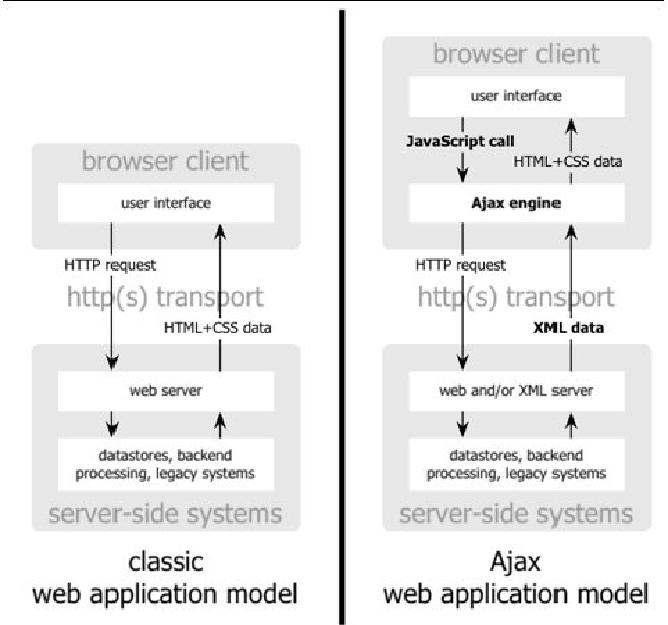
\includegraphics[scale=.7, keepaspectratio=true]{imagenes/02_imagen.png}
\caption{Tecnolog\'ias agrupadas bajo el concepto de AJAX. Fuente: Javier Egu\'iluz P\'erez; \textit{Introducci\'on a AJAX}.}
\end{figure}

En las aplicaciones web tradicionales, las acciones del usuario en la p\'agina (clic en un bot\'on, seleccionar un valor de una lista, etc.) desencadenan llamadas al servidor. Una vez procesada la petici\'on del usuario, el servidor devuelve una nueva p\'agina HTML al navegador del usuario.\\
AJAX permite mejorar completamente la interacci\'on del usuario con la aplicaci\'on, evitando las recargas constantes de la p\'agina, ya que el intercambio de informaci\'on con el servidor se produce en un segundo plano.\\
Las aplicaciones construidas con AJAX eliminan la recarga constante de p\'aginas mediante la creaci\'on de un elemento intermedio entre el usuario y el servidor. La nueva capa intermedia de AJAX mejora la respuesta de la aplicaci\'on. Adem\'as que otorga cierta elegancia a la forma de responder de la pagina frente a las acciones del usuario.






\section{Hyper Text Markup Language (HTML)}
Hyper Text Markup Language (Lenguaje de Marcado de Hipertexto), o HTML, es el lenguaje de marcado predominante para la elaboraci\'on de p\'aginas web. Es usado para describir la estructura y el contenido en forma de texto, as\'i como para complementar el texto con otros elementos.\\
HTML tambi\'en es usado para referirse al contenido del tipo de MIME text/html o como un t\'ermino gen\'erico para el HTML, ya sea en forma descendida del XML (como XHTML 1.0 y posteriores) o en forma descendida directamente de SGML (como HTML 4.01 y anteriores).
Este lenguaje ser\'a el encargado de convertir un simple archivo de texto inicial en una p\'agina web con diferentes tipos y tama\~nos de letra, con im\'agenes, animaciones, formularios interactivos, etc \cite{html}.

\section{eXtensible Markup Language (XML)}
``\textit{Es un metalenguaje de etiquetas extensible desarrollado por la W3C. Consolidado como una simplificaci\'on y adaptaci\'on del SGML que permite definir la gram\'atica de lenguajes espec\'ificos (de la misma manera que HTML es a su vez un lenguaje definido por SGML). Por lo tanto XML no es realmente un lenguaje en particular, sino una manera de definir lenguajes para diferentes necesidades. Algunos de estos lenguajes que usan XML para su definici\'on son XHTML, SVG, MathML.}''. \cite{xml}
XML no ha nacido s\'olo para su aplicaci\'on en Internet, sino que se propone como un est\'andar para el intercambio de informaci\'on estructurada entre diferentes plataformas. Se puede usar en bases de datos, editores de texto, hojas de c\'alculo y casi cualquier cosa imaginable.\\
XML tiene un papel muy importante en la actualidad ya que permite la compatibilidad entre sistemas para compartir la informaci\'on de una manera segura, fiable y f\'acil.\\
La principal que se tiene al utilizar XML es que nos es posible estructurar la informaci\'on para distintos prop\'ositos.

\section{Hojas de Estilo (CSS)}
CSS es un lenguaje creado para controlar el aspecto o presentaci\'on de los documentos electr\'onicos definidos con HTML y XHTML. CSS es la mejor forma de separar los contenidos y su presentaci\'on y es imprescindible para crear p\'aginas web complejas.\\
``\textit{Separar la definici\'on de los contenidos y la definici\'on de su aspecto presenta numerosas ventajas, ya que obliga a crear documentos HTML/XHTML bien definidos y con significado completo (tambi\'en llamados "documentos sem\'anticos")}''. Adem\'as, mejora la accesibilidad del documento, reduce la complejidad de su mantenimiento y permite visualizar el mismo documento en infinidad de dispositivos diferentes \cite{css}.
Al crear una p\'agina web, se utiliza en primer lugar el lenguaje HTML/XHTML para marcar  los contenidos, es decir, para designar la funci\'on de cada elemento dentro de la p\'agina: p\'arrafo, titular, texto destacado, tabla, lista de elementos, etc.\\
Una vez creados los contenidos, se utiliza el lenguaje CSS para definir el aspecto de cada elemento: color, tama\~no y tipo de letra del texto, separaci\'on horizontal y vertical entre elementos,  posici\'on de cada elemento dentro de la p\'agina, etc.\\
Todo este trabajo se logra definiendo caracter\'isticas en el HTML conocidas como atributos, pero no cualquier atributo, concretamente el atributo ``class'' o tambi\'en el atributo ``id'', el primero de uso exclusivo para las hojas de estilo (CSS), y el segundo como una alternativa, el atributo ``id'' tambi\'en es utilizado frecuentemente en las instrucciones de Javascript.

\section{JavaScript}
El JavaScript es un lenguaje de programaci\'on que surgi\'o por la necesidad de ampliar las posibilidades del HTML. En efecto, al poco tiempo de que las p\'aginas web apareciesen, se hizo patente la necesidad de algo m\'as que las limitadas prestaciones del lenguaje b\'asico, ya que el HTML solamente provee de elementos que act\'uan exclusivamente sobre el texto y su estilo, pero no permite, como ejemplo sencillo, ni siquiera abrir una nueva ventana o emitir un mensaje de aviso.\\
JavaScript  se utiliza principalmente para crear p\'aginas web din\'amicas.\\
Una p\'agina web din\'amica es aquella que incorpora efectos como texto que aparece y desaparece, animaciones, acciones que se activan al pulsar botones y ventanas con mensajes de aviso al usuario.\\
T\'ecnicamente, JavaScript es un lenguaje de programaci\'on interpretado, por lo que no es necesario compilar los programas para ejecutarlos. En otras palabras, los programas escritos con JavaScript se pueden probar directamente en cualquier navegador sin necesidad de procesos intermedios. \cite{js}

\section{Hypertext Pre-Processor (PHP)}
PHP es un lenguaje de programaci\'on usado normalmente para la creaci\'on de p\'aginas web din\'amicas. Se trata de un lenguaje interpretado.\\
Su interpretaci\'on y ejecuci\'on se da en el servidor web, en el cual se encuentra almacenado el script, y el cliente s\'olo recibe el resultado de la ejecuci\'on. Cuando el cliente hace una petici\'on al servidor para que le env\'ie una p\'agina web, generada por un script PHP, el servidor ejecuta el int\'erprete de PHP, el cual procesa el script solicitado que generar\'a el contenido de manera din\'amica, pudiendo modificar el contenido al enviar, y regresar el resultado al servidor, el cual se encarga de regres\'arselo al cliente.\\
Permite la conexi\'on a diferentes tipos de servidores de bases de datos tales como MySQL, Postgres, Oracle, ODBC, DB2, Microsoft SQL Server, Firebird y SQLite; lo cual permite la creaci\'on de Aplicaciones web muy robustas.\\
Tiene la capacidad de ser ejecutado en la mayor\'ia de los sistemas operativos, tales como UNIX (y de ese tipo, como Linux o Mac OS X) y Windows, puede interactuar con los servidores de web m\'as populares ya que existe en versi\'on CGI, m\'odulo para Apache, e ISAPI.\\
PHP es una alternativa a las tecnolog\'ias de Microsoft ASP y ASP.NET (que utiliza C\#/VB.NET como lenguajes), a ColdFusion de la compa\~n\'ia Adobe (antes Macromedia), a JSP/Java de Sun Microsystems, y a CGI/Perl. Aunque su creaci\'on y desarrollo se da en el \'ambito de los sistemas libres, bajo la licencia GNU. \cite{php}
\linebreak
Ventajas
\begin{itemize}
\item Es un lenguaje multiplataforma.
\item Capacidad de conexi\'on con la mayor\'ia de los manejadores de base de datos que se utilizan en la actualidad, destaca su conectividad con MySQL.
\item Capacidad de expandir su potencial utilizando la enorme cantidad de m\'odulos (llamados ext's o extensiones).
\item Posee una amplia documentaci\'on en su p\'agina oficial, entre la cual se destaca que todas las funciones del sistema est\'an explicadas y ejemplificadas en un \'unico archivo de ayuda.
\item Es libre, por lo que se presenta como una alternativa de f\'acil acceso para todos.
\item Permite las t\'ecnicas de Programaci\'on Orientada a Objetos.
\item Biblioteca nativa de funciones sumamente amplia e incluida.
\item No requiere definici\'on de tipos de variables.
\item Tiene manejo de excepciones.
\end{itemize}
Desventajas
\begin{itemize}
\item No posee una abstracci\'on de base de datos est\'andar, sino bibliotecas especializadas para cada motor (a veces m\'as de una para el mismo motor).
\item No posee adecuado manejo de internacionalizaci\'on, unicode, etc.
\end{itemize}

\section{Servidor HTTP Apache}
Apache es el servidor web hecho por excelencia, su configurabilidad, robustez y estabilidad hacen que cada vez millones de servidores reiteren su confianza en este programa.\\
La historia de Apache se remonta a febrero de 1995, donde empieza el proyecto del grupo Apache, el cual est\'a basado en el servidor Apache httpd de la aplicaci\'on original de NCSA.\\
El desarrollo de esta aplicaci\'on original se estanc\'o por alg\'un tiempo tras la marcha de Rob McCool por lo que varios webmaster siguieron creando sus parches para sus servidores web hasta que se contactaron v\'ia email para seguir en conjunto el mantenimiento del servidor web, fue ah\'i cuando formaron el grupo Apache. \cite{apache_server}
Fueron Brian Behlendorf y Cliff Skolnick quienes a trav\'es de una lista de correo coordinaron el trabajo y lograron establecer un espacio compartido de libre acceso para los desarrolladores.\\
Este software libre es grandemente reconocido en muchos \'ambitos empresariales y tecnol\'ogicos, por los siguientes aspectos: 
\begin{itemize}
\item Corre en una multitud de Sistemas Operativos, lo que lo hace pr\'acticamente universal.
\item Apache es una tecnolog\'ia gratuita de c\'odigo fuente abierto. Esto le da una transparencia a este software de manera que si queremos ver que es lo que estamos instalando como servidor , lo podemos saber, sin ning\'un secreto.
\item Apache es un servidor altamente configurable de dise\~no modular. Es muy sencillo ampliar las capacidades de servidor. Actualmente existen muchos m\'odulos para Apache que son adaptables a este, y est\'an ah\'i para que los instalemos cuando los necesitemos. 
\item Apache trabaja con gran cantidad de lenguajes como Perl, PHP y otros lenguajes de script. Teniendo todo el soporte que se necesita para tener p\'aginas din\'amicas.
\item Apache te permite personalizar la respuesta ante los posibles errores que se puedan dar en el servidor. Es posible configurar Apache para que ejecute un determinado script cuando ocurra un error en concreto.
\item Tiene una alta configurabilidad en la creaci\'on y gesti\'on de logs. Apache permite la creaci\'on de ficheros de log a medida.
\end{itemize}

\section{MySQL}
MySQL es un sistema gestor de bases de datos relacionales en SQL, esto significa que permite la gesti\'on de los datos de una Base de datos relacional, usando un lenguaje de consulta estructurado. Y, por tanto, que a partir de una oraci\'on llamada m\'as propiamente consulta, MySQL llevar\'a a cabo una determinada acci\'on sobre nuestra base de datos. \cite{mysql_server}
Algunas de sus caracter\'isticas son:
\begin{itemize}
\item C\'odigo abierto
\item F\'acil de instalar y configurar
\item Funcionalidad
\item Portabilidad
\item Velocidad
\end{itemize}

\section{Programaci\'on orientada a objetos}
El desarrollo de software es un proceso muy complejo que requiere de una metodolog\'ia eficiente y sistem\'atica. El ciclo de vida de un sistema de computaci\'on comienza con la formulaci\'on de un problema, seguido de an\'alisis, dise\~no, implementaci\'on, verificaci\'on y validaci\'on del software. El modelo orientado a objetos presenta un enfoque evolucionado para la ingenier\'ia de software.\\
Una diferencia importante entre la programaci\'on tradicional y la programaci\'on orientada a objetos es que la programaci\'on tradicional separa los datos de las funciones, mientras que la programaci\'on orientada a objetos define un conjunto de objetos donde se combina de forma modular los datos con las funciones. \cite{poo_deitel}
Los aspectos principales de la programaci\'on orientada a objetos son:
\begin{itemize}
\item Objetos
\item Clasificaci\'on
\item Instanciaci\'on
\item Generalizaci\'on
\item Abstracci\'on
\item Encapsulaci\'on
\item Modularidad
\item Extensibilidad
\item Polimorfismo
\item Reutilizaci\'on de C\'odigo
\end{itemize}

\section{UML}
UML (Unified Modeling Language) es un lenguaje que permite modelar, construir y documentar los elementos que forman un sistema o software orientado a objetos. Se ha convertido en el est\'andar de facto de la industria, debido a que ha sido concebido por los autores de los tres m\'etodos m\'as usados de orientaci\'on a objetos: Grady Booch, Ivar Jacobson y Jim Rumbaugh.\\
Esta notaci\'on ha sido ampliamente aceptada debido al prestigio de sus creadores y debido a que incorpora las principales ventajas de cada uno de los m\'etodos particulares en los que se basa.\\
Booch, OMT y OOSE. UML ha puesto fin a las llamadas ``guerras de m\'etodos'' que se han mantenido a lo largo de los 90, en las que los principales m\'etodos sacaban nuevas versiones que incorporaban las t\'ecnicas de los dem\'as. Con UML se fusiona la notaci\'on de estas t\'ecnicas para formar una herramienta compartida entre todos los ingenieros software que trabajan en el desarrollo orientado a objetos.\\
El objetivo principal cuando se empez\'o a gestar UML era posibilitar el intercambio de modelos entre las distintas herramientas CASE orientadas a objetos del mercado. Hay que tener en cuenta que el est\'andar UML no define un proceso de desarrollo espec\'ifico, tan solo se trata de una notaci\'on. \cite{ing_soft}

\section{Patrones Arquitect\'onicos}
Los patrones arquitect\'onicos se utilizan principalmente para definir la arquitectura (estructura) de la aplicaci\'on de software. El objetivo de utilizar estos patrones es mejorar tanto el rendimiento como la mantenibilidad de los sistemas inform\'aticos\cite{design_patterns}.

\subsection{MVC}
El patr\'on MVC ``\emph{Modelo Vista Controlador}'', define tres elementos b\'asicos de toda aplicaci\'on de software:
\begin{itemize}
\item[Modelo], Los modelos representan a todo lo relacionado con las bases de datos.
\item[Vista], Las vistas representan a las pantallas finales para el usuario.
\item[Controlador], Los controladores, como su nombre indica, se concentran en las acciones que se generan desde las vistas para procesarlas.
\end{itemize}

\subsection{MVP}
El patr\'on MVP ``\emph{Modelo Vista Presentador}'', es muy similar al MVC, de hecho surge como una mejora al mencionado patr\'on, tambi\'en define tres elementos b\'asicos de toda aplicaci\'on de software:
\begin{itemize}
\item[Modelo], Los modelos representan a todo lo relacionado con las bases de datos.
\item[Vista], Las vistas representan a las pantallas finales para el usuario.
\item[Presentador], Los presentadores hacen de controladores, pero a la vez se encargan de presentar la informaci\'on necesaria a las vistas, para que estas se construyan.
\end{itemize}

\begin{figure}[h]
\centering
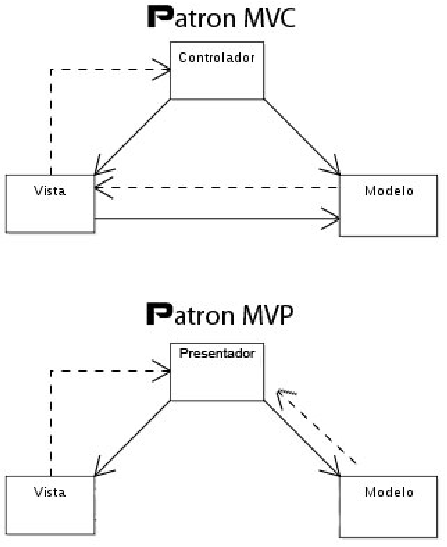
\includegraphics[scale=.7, keepaspectratio=true]{imagenes/11_imagen.png}
\caption{Patr\'ones MVC vs MVP.}
\end{figure}

\section{Otros Patrones}
Aparte de los patrones de arquitectura, existen muchos otros patrones que proveen soluciones a problemas casi cotidianos en el desarrollo de cualquier sistema tanto web como de escritorio \cite{design_patterns}.

A continuaci\'on se presentan algunos de ellos.

\subsection{Patr\'on Singleton}
Este patr\'on es uno de los m\'as b\'asicos y tambi\'en uno de los m\'as utilizados en los Sitemas de Informaci\'on. Consiste en tener una sola instancia de alguna clase la cual es global para toda la aplicaci\'on.

\subsection{Patr\'on Factory Method}
Este patr\'on fue utilizado para complementar el patr\'on Singleton. Consiste en tener una clase con m\'etodos que se encargan de construir instancias de distintas clases.

\section{Sistemas de Informaci\'on Web}
La principal caracter\'istica que tiene un sistema de informaci\'on web frente a un sistema de informaci\'on tradicional es que un sistema de informaci\'on web, est\'a alojado en un servidor web, por tanto es posible acceder a \'el desde cualquier parte del mundo, las 24 horas del d\'ia y desde cualquier equipo que tenga conexi\'on a internet, en cambio con un sistema tradicional accedemos a \'el, desde un terminal especifico.\\
Otra ventaja que se tiene en un sistema web es que la informaci\'on almacenada en el servidor ya tiene sus propios respaldos y dem\'as, gracias a las pol\'iticas manejadas por los due\~nos de  los servidores. De esta manera deja de ser una preocupaci\'on para el usuario final el c\'omo evitar la p\'erdida o corrupci\'on de la informaci\'on.

\clearpage
